\documentclass{experimentreport}

\usepackage{graphicx}
\usepackage{booktabs}
\input{listing_style.tex}

%========================
% Basic Information
%========================

\setcoursename{Practical Techniques in Fundamental Software Development: Intelligent Software Engineering}
\setreportname{Intelligent Software Engineering Experiment Report}

\setexperimenttitle{Experiment 1: Mining Code Review Comments and Understanding Requirements}

\setstudentname{Marlen Melis}
\setdepartment{School of Computing}
\setstudentid{2026140428}

\setcourseteacher{Liu Jiakun}
\setinstructor{Liu Jiakun}

\setlablocation{Dormitory}
\setlabtime{Evening}

\begin{document}

%========================
% Automatically Generate Cover Page
%========================

\makereporthead

%========================
% Experiment Objectives
%========================

\experimentpurpose{

Upon completion of this experiment, I am able to:

\begin{enumerate}
\item Understand the basic workflow of Pull Requests (PRs) and code reviews in modern software development (fork $\rightarrow$ commit $\rightarrow$ open PR $\rightarrow$ review $\rightarrow$ discuss $\rightarrow$ merge/close).
\item Explain how code review data is organized inside a real GitHub open-source repository, across five actively-maintained projects spanning three languages.
\item State the relationships between Pull Requests, Commits, Reviews, Review Comments, Issue Comments, and Labels, and represent them as seven linked flat tables.
\item Retrieve code review data at scale using the authenticated GitHub GraphQL and REST APIs, with on-disk caching for idempotent, resumable mining.
\item Extract multi-source information --- code diffs, commit messages, PR text, and structured metadata --- for every mined Pull Request.
\item Apply statistical analysis and visualization to the resulting dataset, and use it to establish an explicit, evidence-based data foundation (including a documented class-imbalance report) for the machine-learning and LLM experiments that follow.
\end{enumerate}

}

%========================
% Experiment Content
%========================

\experimentcontent{

\subsection*{1. Repositories and Sampling Strategy}

Five large, actively-maintained open-source repositories were selected, chosen so that each had a
verifiable population of AI-authored Pull Requests (queried live against GitHub's search API
before finalizing the shortlist, rather than assumed):
\texttt{microsoft/vscode} (TypeScript), \texttt{dotnet/runtime} and \texttt{dotnet/aspnetcore}
(C\#), \texttt{microsoft/semantic-kernel} (Python/C\#), and \texttt{home-assistant/core} (Python).

A pure random sample of 300 closed PRs per repository would contain few or zero AI-authored PRs
by chance, since AI-authored PRs are a small minority of all PRs in most repositories. The
sampling strategy therefore, per repository: (1) searched for PRs authored by GitHub's own
Copilot coding agent (\texttt{is:closed author:app/copilot-swe-agent}), capped at 100; (2) filled
the remaining slots with a sample of recent closed PRs, skipping any overlap with step 1. This
deliberately over-represents AI-authored PRs relative to their natural base rate --- a documented
design decision, not a hidden shortcut. Only closed PRs were targeted, so every sampled PR has a
final merge/close label.

\subsection*{2. Mining Pipeline}

An authenticated GitHub client (\texttt{src/mining/github\_client.py}) combines one nested
GraphQL query per PR --- core fields, commits, reviews and their inline comments, top-level issue
comments, and labels --- with paginated REST calls for file-level diff patches, since GraphQL
exposes no unified-diff field. Every raw PR response is cached to disk as JSON, keyed by
\texttt{(owner, repo, number)}, making the mining job idempotent and resumable: re-running only
fetches PRs still missing from the cache. Requests are retried with exponential backoff and
jitter on HTTP 403/429/5xx, and separately on GraphQL-level rate-limit errors (which GitHub
returns as HTTP 200 with an \texttt{errors} array, not an HTTP error code). PRs are fetched
concurrently via a thread pool (10 workers), giving roughly an order of magnitude better
throughput than sequential fetching.

\subsection*{3. AI-Authorship and AI-Reviewer Detection}

Detection (\texttt{src/mining/ai\_detection.py}) uses a three-tier signal hierarchy rather than a
username heuristic:

\begin{enumerate}
\item \textbf{Structural primary signal}: GitHub's GraphQL API tags every actor with
\texttt{\_\_typename} of \texttt{Bot} or \texttt{User} directly.
\item \textbf{Semantic sub-classification of Bot actors}: \texttt{Bot}-typed actors are matched
against curated allowlists of AI coding agents (e.g.\ \texttt{copilot-swe-agent}) and AI review
bots (e.g.\ \texttt{copilot-pull-request-reviewer}, \texttt{coderabbitai}). Non-AI automation
(\texttt{dependabot}, \texttt{renovate}, \texttt{github-actions}, \ldots) is excluded explicitly;
anything \texttt{Bot}-typed but on neither AI list is reported honestly as \texttt{other\_bot}
rather than guessed into an AI category.
\item \textbf{Secondary, lower-confidence signal}: for PRs opened by a human whose commit trail
still shows AI involvement --- an agent commit identity/no-reply email pattern, or Copilot's
literal \texttt{"Initial plan"} placeholder first commit --- flagged as a distinct
\texttt{human\_opened\_ai\_assisted} category at explicitly lower confidence than a fully
agent-authored PR.
\end{enumerate}

Every detection carries a \texttt{method}, a \texttt{confidence}, and human-readable
\texttt{evidence}, so it can be spot-checked rather than trusted blindly. A manual precision
review was performed on 59 distinct flagged PRs (a random sample of 40, plus a full census of all
19 PRs flagged only by the weaker secondary signal); zero false positives were found (Section
``Experimental Results'' below).

\subsection*{4. Data Model and Statistical Analysis}

Mined PRs are flattened into seven parquet tables --- \texttt{pull\_requests}, \texttt{commits},
\texttt{files\_changed}, \texttt{reviews}, \texttt{review\_comments}, \texttt{issue\_comments},
\texttt{ai\_signals} --- with AI-detection flags folded directly onto \texttt{pull\_requests} as
well as kept in their own table. \texttt{src/mining/analyze\_exp1.py} computes descriptive
statistics and generates visualizations for every measure the lab guide asks for --- merge status,
review-comment-count distribution, reviewer-count distribution, PR-length distribution, label
distribution, AI-vs-human PR counts, and AI-reviewer presence --- broken out \emph{per repository
and pooled}, since a pooled-only number can hide very different per-repository behavior.

}

%========================
% Experiment Results
%========================

\experimentresult{

\subsection*{1. Samples of Successfully Retrieved Pull Request Data}

\begin{center}
\begin{tabular}{|l|r|p{5.4cm}|l|c|r|r|}
\hline
\textbf{Repo} & \textbf{\#} & \textbf{Title} & \textbf{Author} & \textbf{Merged} & \textbf{+lines} & \textbf{--lines} \\
\hline
microsoft/vscode & 326979 & dictation: publish native runtime to CDN instead of\ldots & meganrogge (human) & Yes & 1232 & 141 \\
\hline
microsoft/vscode & 326697 & Fix Cmd/Ctrl+I dictation in the Agents window composer & copilot-swe-agent (AI) & Yes & 128 & 73 \\
\hline
\end{tabular}
\end{center}

Every retrieved PR carries: GraphQL node ID, repo, number, title, body, author login/type,
timestamps, state, merge status, additions/deletions/changed-files counts, labels, and the full
AI-detection verdict (\texttt{is\_ai\_authored}, \texttt{ai\_authored\_kind},
\texttt{ai\_authored\_method}, \texttt{ai\_authored\_confidence}, \texttt{is\_ai\_reviewed}).

\subsection*{2. Samples of Successfully Retrieved Review Comments}

\begin{quote}
\textbf{Human reviewer} on \texttt{tests/components/caldav/test\_calendar.py}: \\
``Thanks for the feedback! I'll remove it.''
\end{quote}

\begin{quote}
\textbf{AI reviewer (copilot-pull-request-reviewer)} on
\texttt{homeassistant/components/midea\_lan/config\_flow.py}: \\
``Guard against missing DEFAULT\_CLOUD in the returned cloud server mapping to avoid
StopIteration and a crashed config flow.''
\end{quote}

\begin{quote}
\textbf{Human reviewer} on \texttt{homeassistant/components/denon\_rs232/media\_player.py}: \\
``Will be modified, along with the same issue at line 79 (for consistency).''
\end{quote}

Even from three examples, a qualitative pattern is visible and is discussed further under
Reflection Question 4: the AI reviewer's comment is a single, self-contained technical
observation with a concrete failure mode named (\texttt{StopIteration}), while the human
comments are conversational turns embedded in a back-and-forth thread.

\subsection*{3. Samples of Successfully Preprocessed Data}

Raw GraphQL/REST responses were flattened into seven linked, parquet-serialized tables:

\begin{center}
\begin{tabular}{|l|r|l|}
\hline
\textbf{Table} & \textbf{Rows} & \textbf{Key} \\
\hline
pull\_requests & 1{,}494 & \texttt{id} (also carries AI-signal flags) \\
commits & 6{,}861 & \texttt{pr\_id} \\
files\_changed & 27{,}110 & \texttt{pr\_id} \\
reviews & 7{,}016 & \texttt{pr\_id}, \texttt{review\_id} \\
review\_comments & 6{,}351 & \texttt{pr\_id}, \texttt{review\_id}, \texttt{comment\_id} \\
issue\_comments & 3{,}183 & \texttt{pr\_id}, \texttt{comment\_id} \\
ai\_signals & 1{,}494 & \texttt{pr\_id} \\
\hline
\end{tabular}
\end{center}

Preprocessing included: normalizing labels from a nested GraphQL connection into a flat list per
PR; de-duplicating PR numbers that appeared twice due to pagination drift on a live, frequently
updated repository listing (one such case was found and fixed --- see ``Summary of Problems
Encountered''); and folding the AI-detection verdict directly onto each PR row.

\subsection*{4. Statistical Results}

\textbf{Dataset size.} 1{,}494 of 1{,}500 targeted PRs were successfully retrieved. The 6-PR
shortfall has two distinct causes, both documented rather than silently dropped: \textbf{5 PRs}
were permanently excluded after exhausting a 6-attempt retry budget on server-side 502 errors
(\texttt{aspnetcore} 1, \texttt{runtime} 1, \texttt{semantic-kernel} 3), and \textbf{1 further slot}
was lost in \texttt{microsoft/vscode} because pagination drift put the same PR on two pages, so that
repo's 300-entry sample list held only 299 \emph{distinct} PRs (see ``Summary of Problems
Encountered'' \#2). Per repository: \texttt{dotnet/aspnetcore} 299, \texttt{dotnet/runtime} 299,
\texttt{home-assistant/core} 300, \texttt{microsoft/semantic-kernel} 297, \texttt{microsoft/vscode}
299.

\textbf{Merged vs.\ non-merged (class balance).} Overall: \textbf{1{,}075 merged / 419 not merged
(72.0\% merge rate)} --- a moderate class imbalance. Per repository the rate ranges from 63.0\%
(\texttt{semantic-kernel}) to 81.9\% (\texttt{dotnet/runtime}), so the imbalance is not uniform
across repositories either. This is discussed directly in Reflection Question 5.

\begin{center}
\begin{tabular}{|l|r|r|r|}
\hline
\textbf{Repo} & \textbf{Merged} & \textbf{Not merged} & \textbf{Merge rate} \\
\hline
dotnet/aspnetcore & 201 & 98 & 67.2\% \\
dotnet/runtime & 245 & 54 & 81.9\% \\
home-assistant/core & 219 & 81 & 73.0\% \\
microsoft/semantic-kernel & 187 & 110 & 63.0\% \\
microsoft/vscode & 223 & 76 & 74.6\% \\
\hline
\textbf{Pooled} & \textbf{1{,}075} & \textbf{419} & \textbf{72.0\%} \\
\hline
\end{tabular}
\end{center}

\textbf{Review-comment-count distribution.} Pooled mean 4.25, median 1, heavily right-skewed
(std 12.4, max 242 on a single \texttt{home-assistant/core} PR); \textbf{701 of 1{,}494 PRs
(46.9\%) received zero inline review comments}. \texttt{home-assistant/core} has both the highest
mean (7.13) and the most extreme outlier; \texttt{microsoft/vscode} the lowest mean (1.77).

\textbf{Reviewer-count distribution.} Pooled mean 2.46 distinct reviewers per PR, median 2,
max 10; 172 PRs (11.5\%) had zero reviewers recorded.

\textbf{PR-length distribution (additions + deletions).} Pooled median 57 lines --- most PRs are
small --- but the mean (17{,}592) is dominated by extreme outliers (max 14{,}285{,}506 lines,
almost certainly a vendored-dependency or lockfile-regeneration commit); the 90th percentile is
only 702 lines. Per-repo medians are similar (36--72 lines) despite very different means, confirming
the skew is driven by a small number of huge PRs, not a systematically different typical PR size
across repos.

\textbf{Label distribution.} 1{,}071 of 1{,}494 PRs (71.7\%) carry at least one label. The pooled
top labels are dominated by \texttt{home-assistant/core}'s heavy labeling conventions
(\texttt{cla-signed} 261, \texttt{small-pr} 169, \texttt{has-tests} 129), while
\texttt{microsoft/vscode} uses labels far more sparingly (top label \texttt{dependencies} at only
12) --- label usage is a per-repository convention, not a universal signal.

\textbf{AI-authored vs.\ human-authored PRs.} Pooled: \textbf{380 AI-authored (25.4\%) vs.\ 1{,}114
human-authored}, but this share varies sharply by repo: 37.5\% in \texttt{aspnetcore} and 36.8\%
in \texttt{dotnet/runtime} vs.\ only 10.3\% in \texttt{home-assistant/core} and 7.7\% in
\texttt{semantic-kernel} --- reflecting how actively each project's maintainers have adopted the
Copilot coding agent, not an inherent property of the codebase. Of the 380 AI-authored PRs, 361
(95.0\%) were detected via the high-confidence allowlist signal (agent account, \texttt{Bot}-typed)
and 19 (5.0\%) via the lower-confidence secondary commit-trail signal --- a genuinely distinct
``human-opened, AI-assisted'' category, close to the $\sim$8\% anticipated at design time.

\textbf{AI-reviewer presence.} Pooled: \textbf{71.2\% of PRs (1{,}064/1{,}494) had at least one AI
reviewer touch them} --- \texttt{copilot-pull-request-reviewer} is present on \emph{all} 1{,}064 of
them, with \texttt{coderabbitai} co-occurring on 4 (never alone: 1{,}060 PRs have Copilot only, 4
have both). Presence ranges from 42.8\% (\texttt{semantic-kernel})
to 86.0\% (\texttt{microsoft/vscode}).

\textbf{Merge rate, AI-authored vs.\ human-authored.} Pooled: AI-authored PRs merge at
\textbf{65.3\%} vs.\ human-authored at \textbf{74.2\%} --- but the direction is \emph{not}
consistent across repositories: in \texttt{dotnet/aspnetcore} (68.8\% vs.\ 66.3\%) and
\texttt{microsoft/semantic-kernel} (69.6\% vs.\ 62.4\%), AI-authored PRs merge \emph{more} often
than human-authored ones, while in \texttt{home-assistant/core} the gap is large and in the
opposite direction (35.5\% vs.\ 77.3\%). Per-repo sample sizes for AI-authored PRs are small in
some repos (\texttt{semantic-kernel} $n=23$, \texttt{home-assistant/core} $n=31$), so these
per-repo rates are noisier than the pooled figure and should be read with that caveat.

\textbf{Manual precision spot-check.} A random sample of 40 flagged PRs plus a full census of the
19 secondary-signal PRs (59 distinct PRs, 68 individual flag assessments) were manually reviewed
against author/reviewer identity, GitHub's structural typing, and --- for the secondary-signal
cases --- the raw commit trail. \textbf{Zero false positives were found} (point-estimate precision
100\%; $\geq\!\sim\!92.5\%$ at 95\% confidence by the rule of three, computed on the 40 random
draws --- the 19-PR census is a full census of the weakest tier, not a random sample, so it
cannot be used to widen that bound). One labeling nuance was
found: a Copilot-authored PR with a deleted (null) author account was correctly flagged
\texttt{is\_ai\_authored=True} but mis-categorized as \texttt{human\_opened\_ai\_assisted} rather
than ``author unknown'' --- an honest, reportable edge case, not an authorship error.

\subsection*{5. Results of the Visual Analysis}

\begin{center}
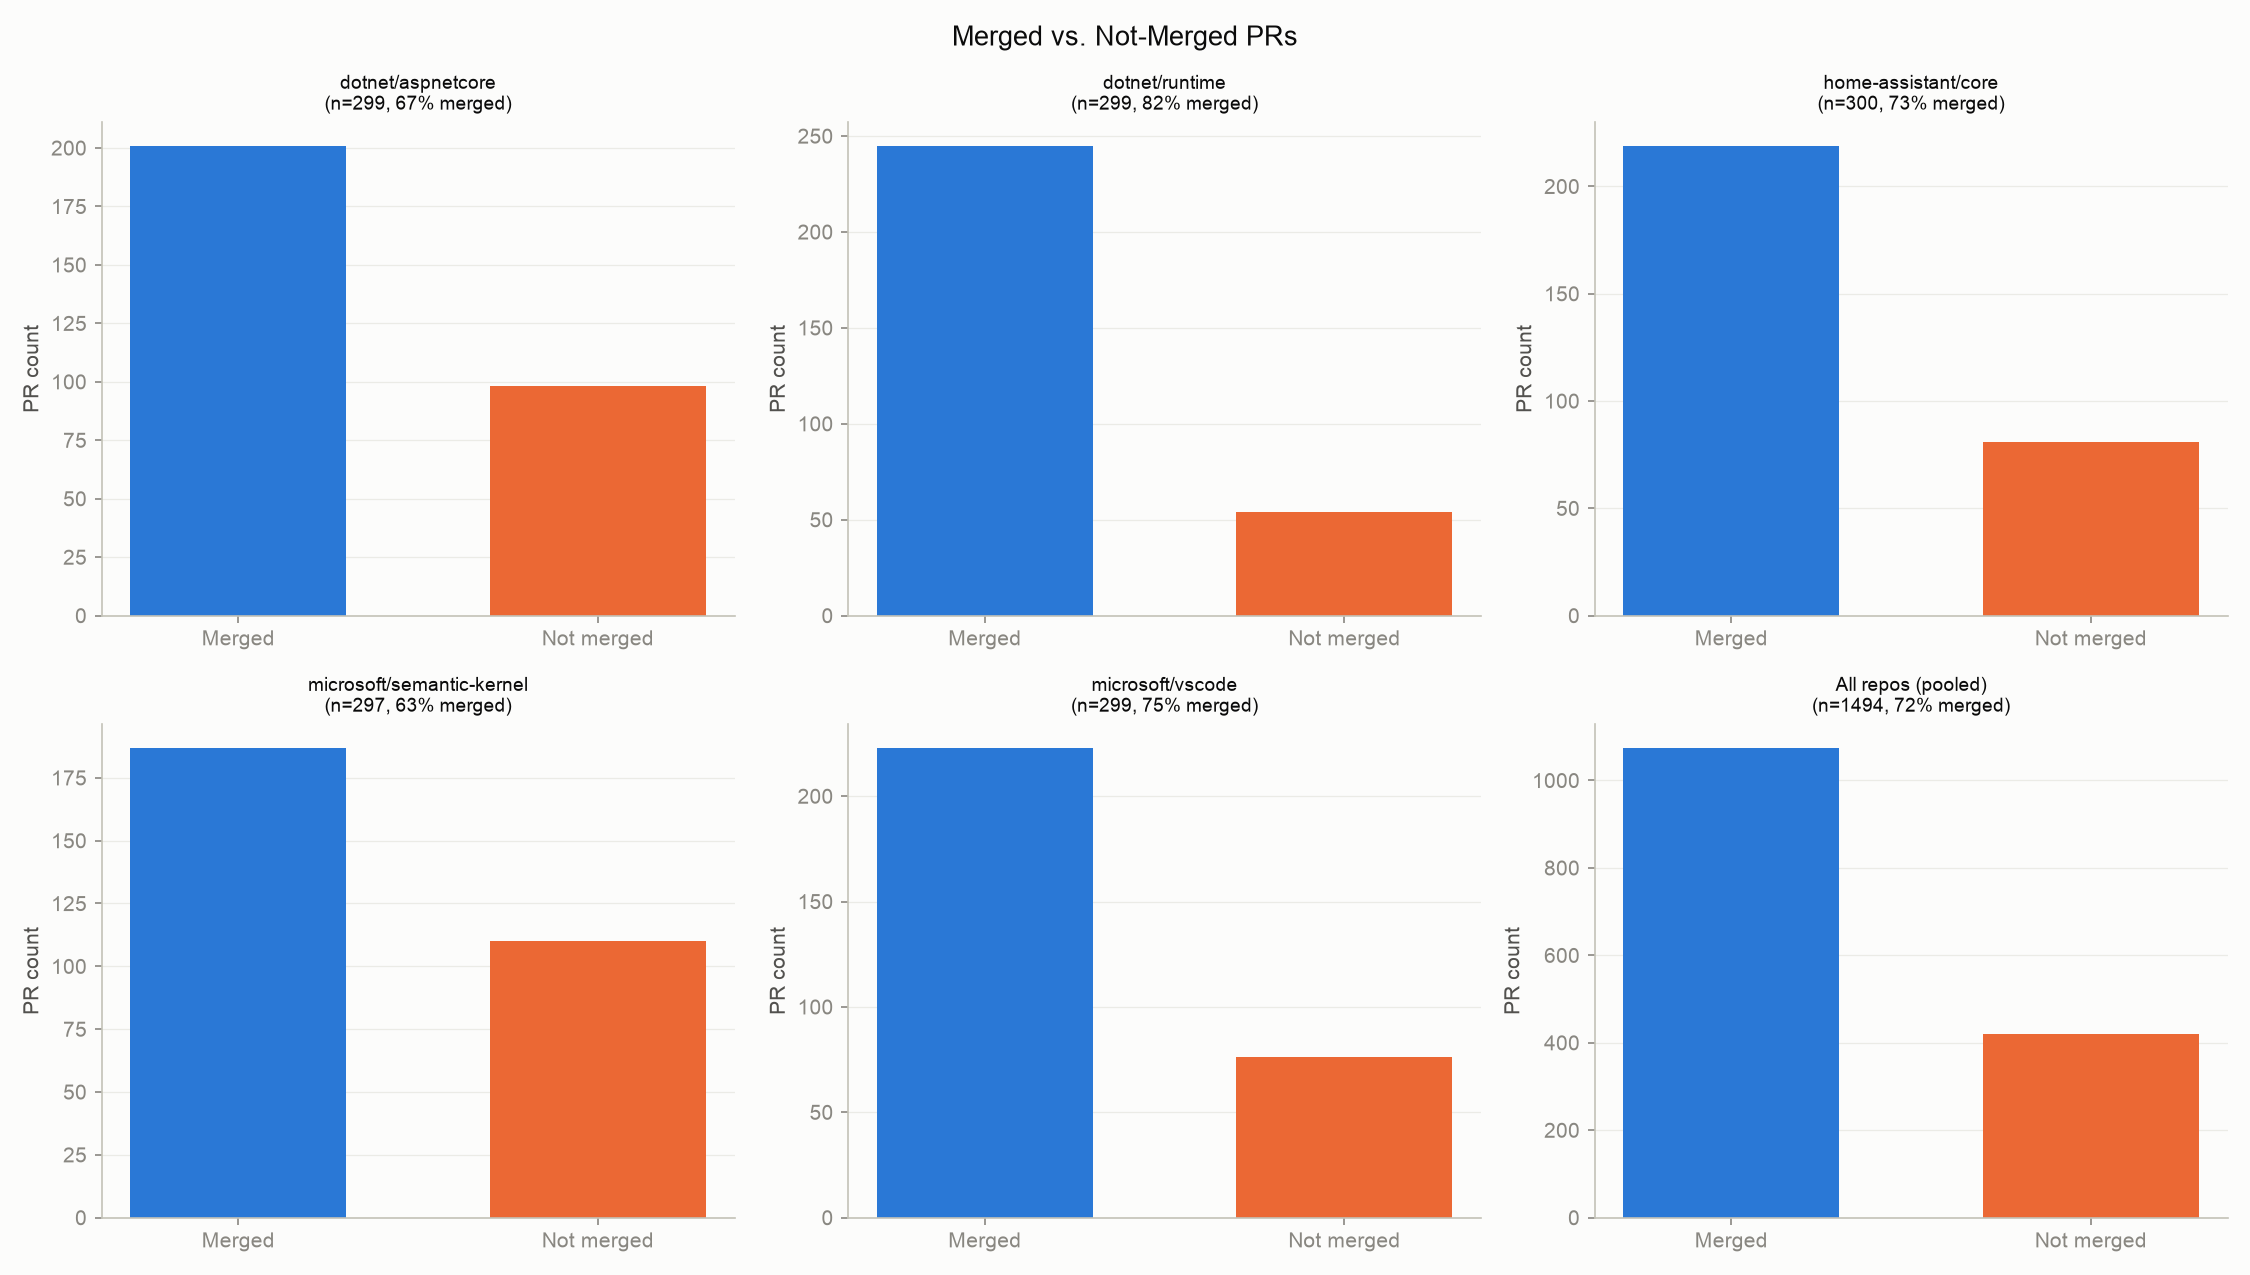
\includegraphics[width=0.92\textwidth]{../results/figures/merge_status.png}
\end{center}
\noindent\textbf{Figure 1.} Merged vs.\ not-merged PR counts, per repo and pooled. Confirms the
72.0\% pooled merge rate and shows every repo individually clears majority-merged, with
\texttt{semantic-kernel} the closest to balanced (63.0\%/37.0\%).

\begin{center}
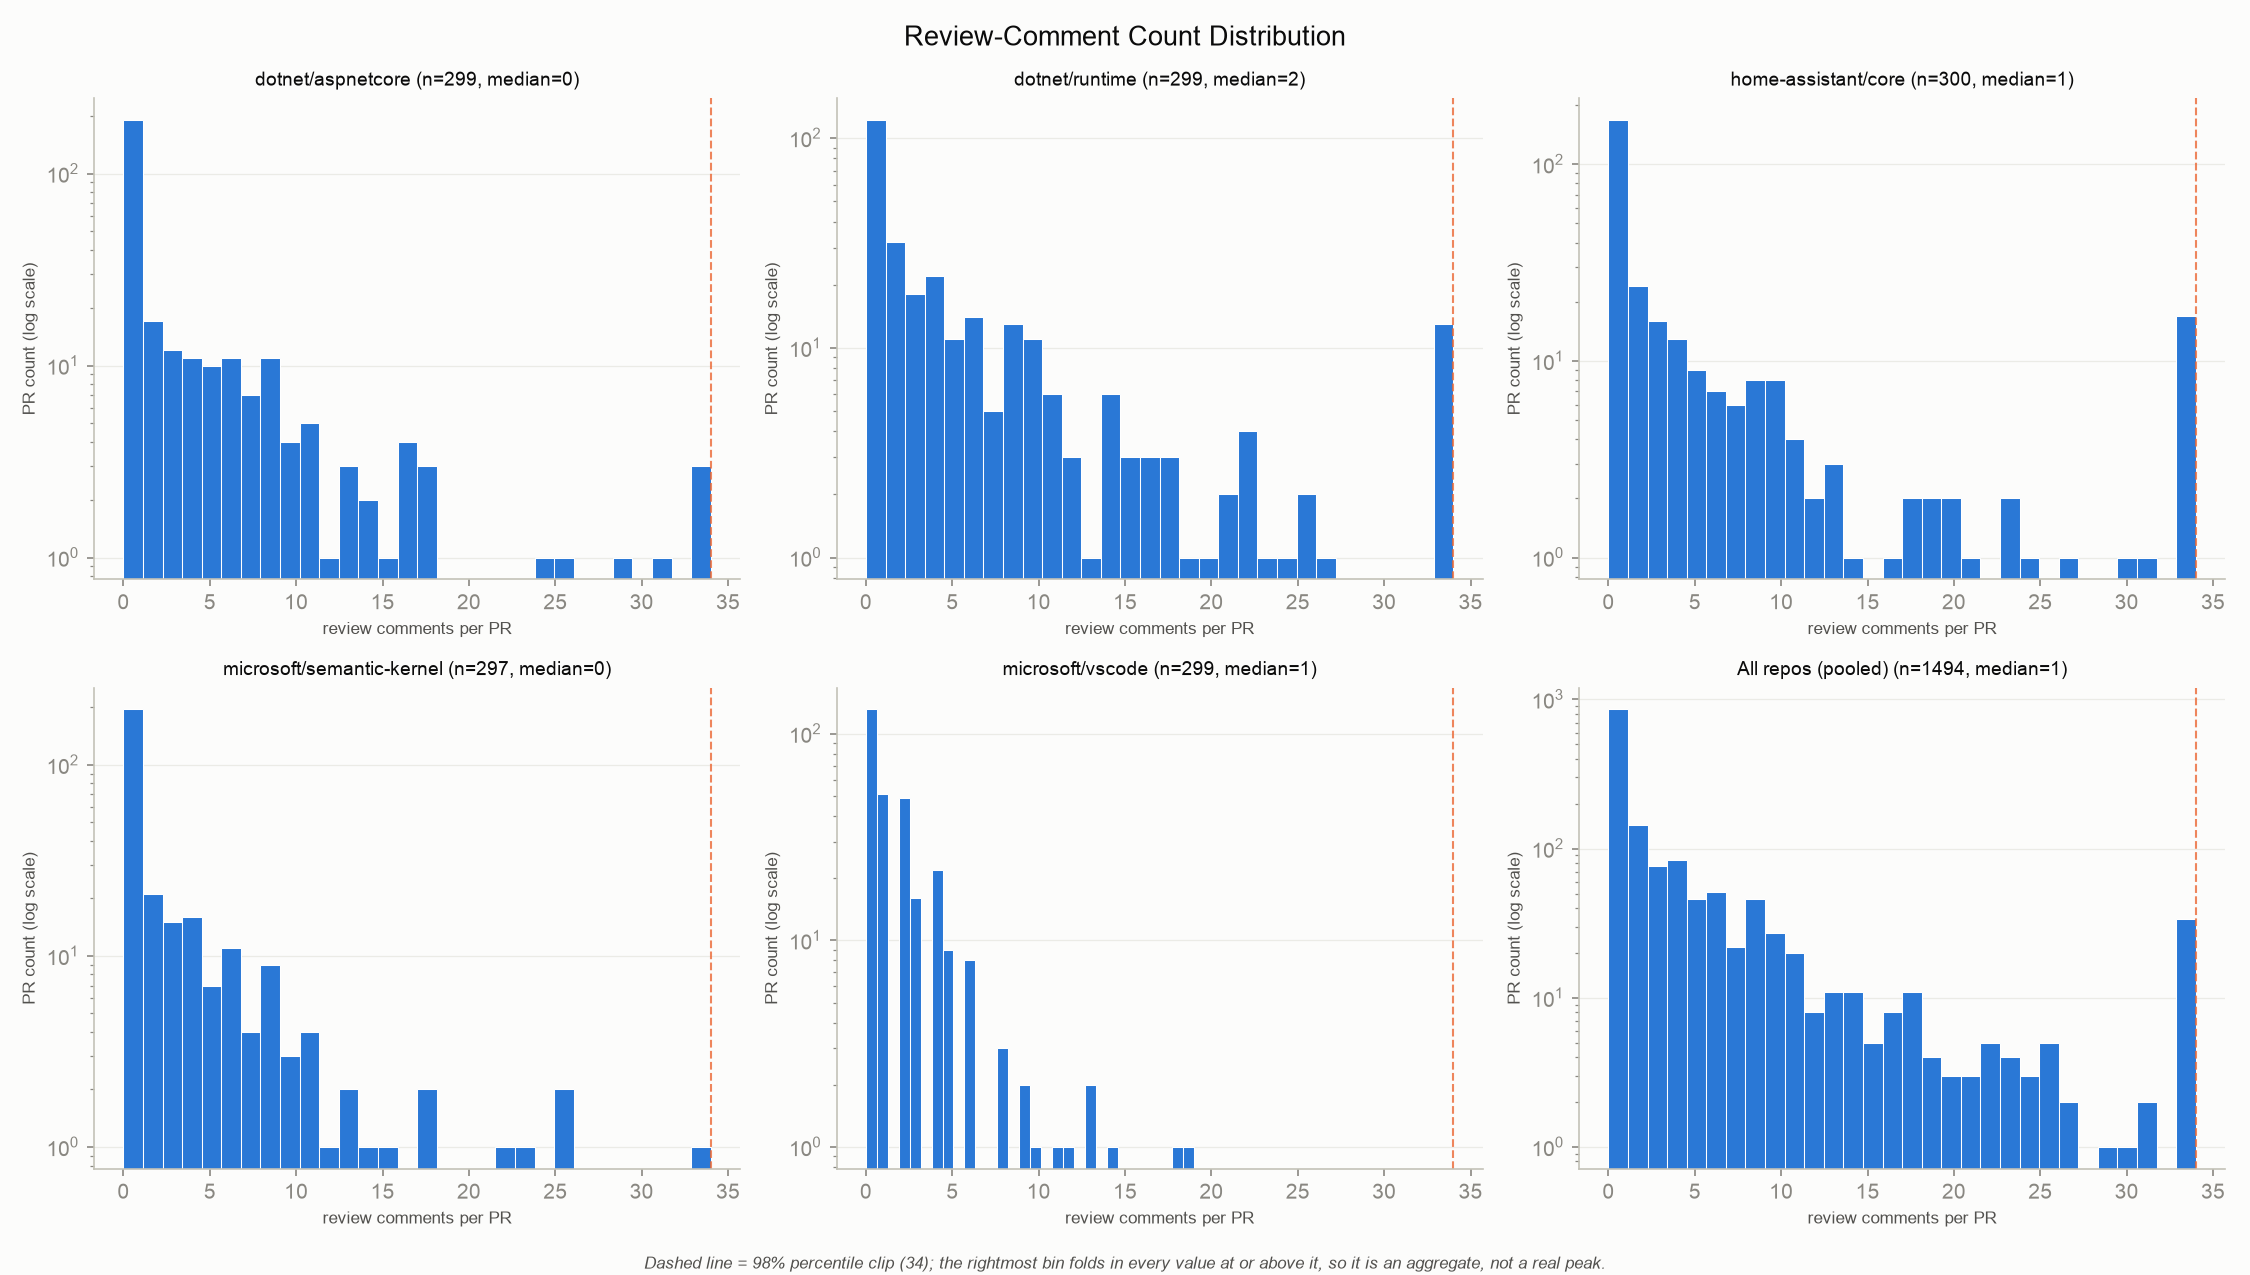
\includegraphics[width=0.92\textwidth]{../results/figures/review_comment_count_distribution.png}
\end{center}
\noindent\textbf{Figure 2.} Review-comment-count distribution (log-scale y, clipped at the 98th
percentile with the clip boundary marked --- the rightmost bin is an aggregate of extreme values,
not a real peak). Confirms the heavy right skew and the near-half of PRs with zero comments.

\begin{center}
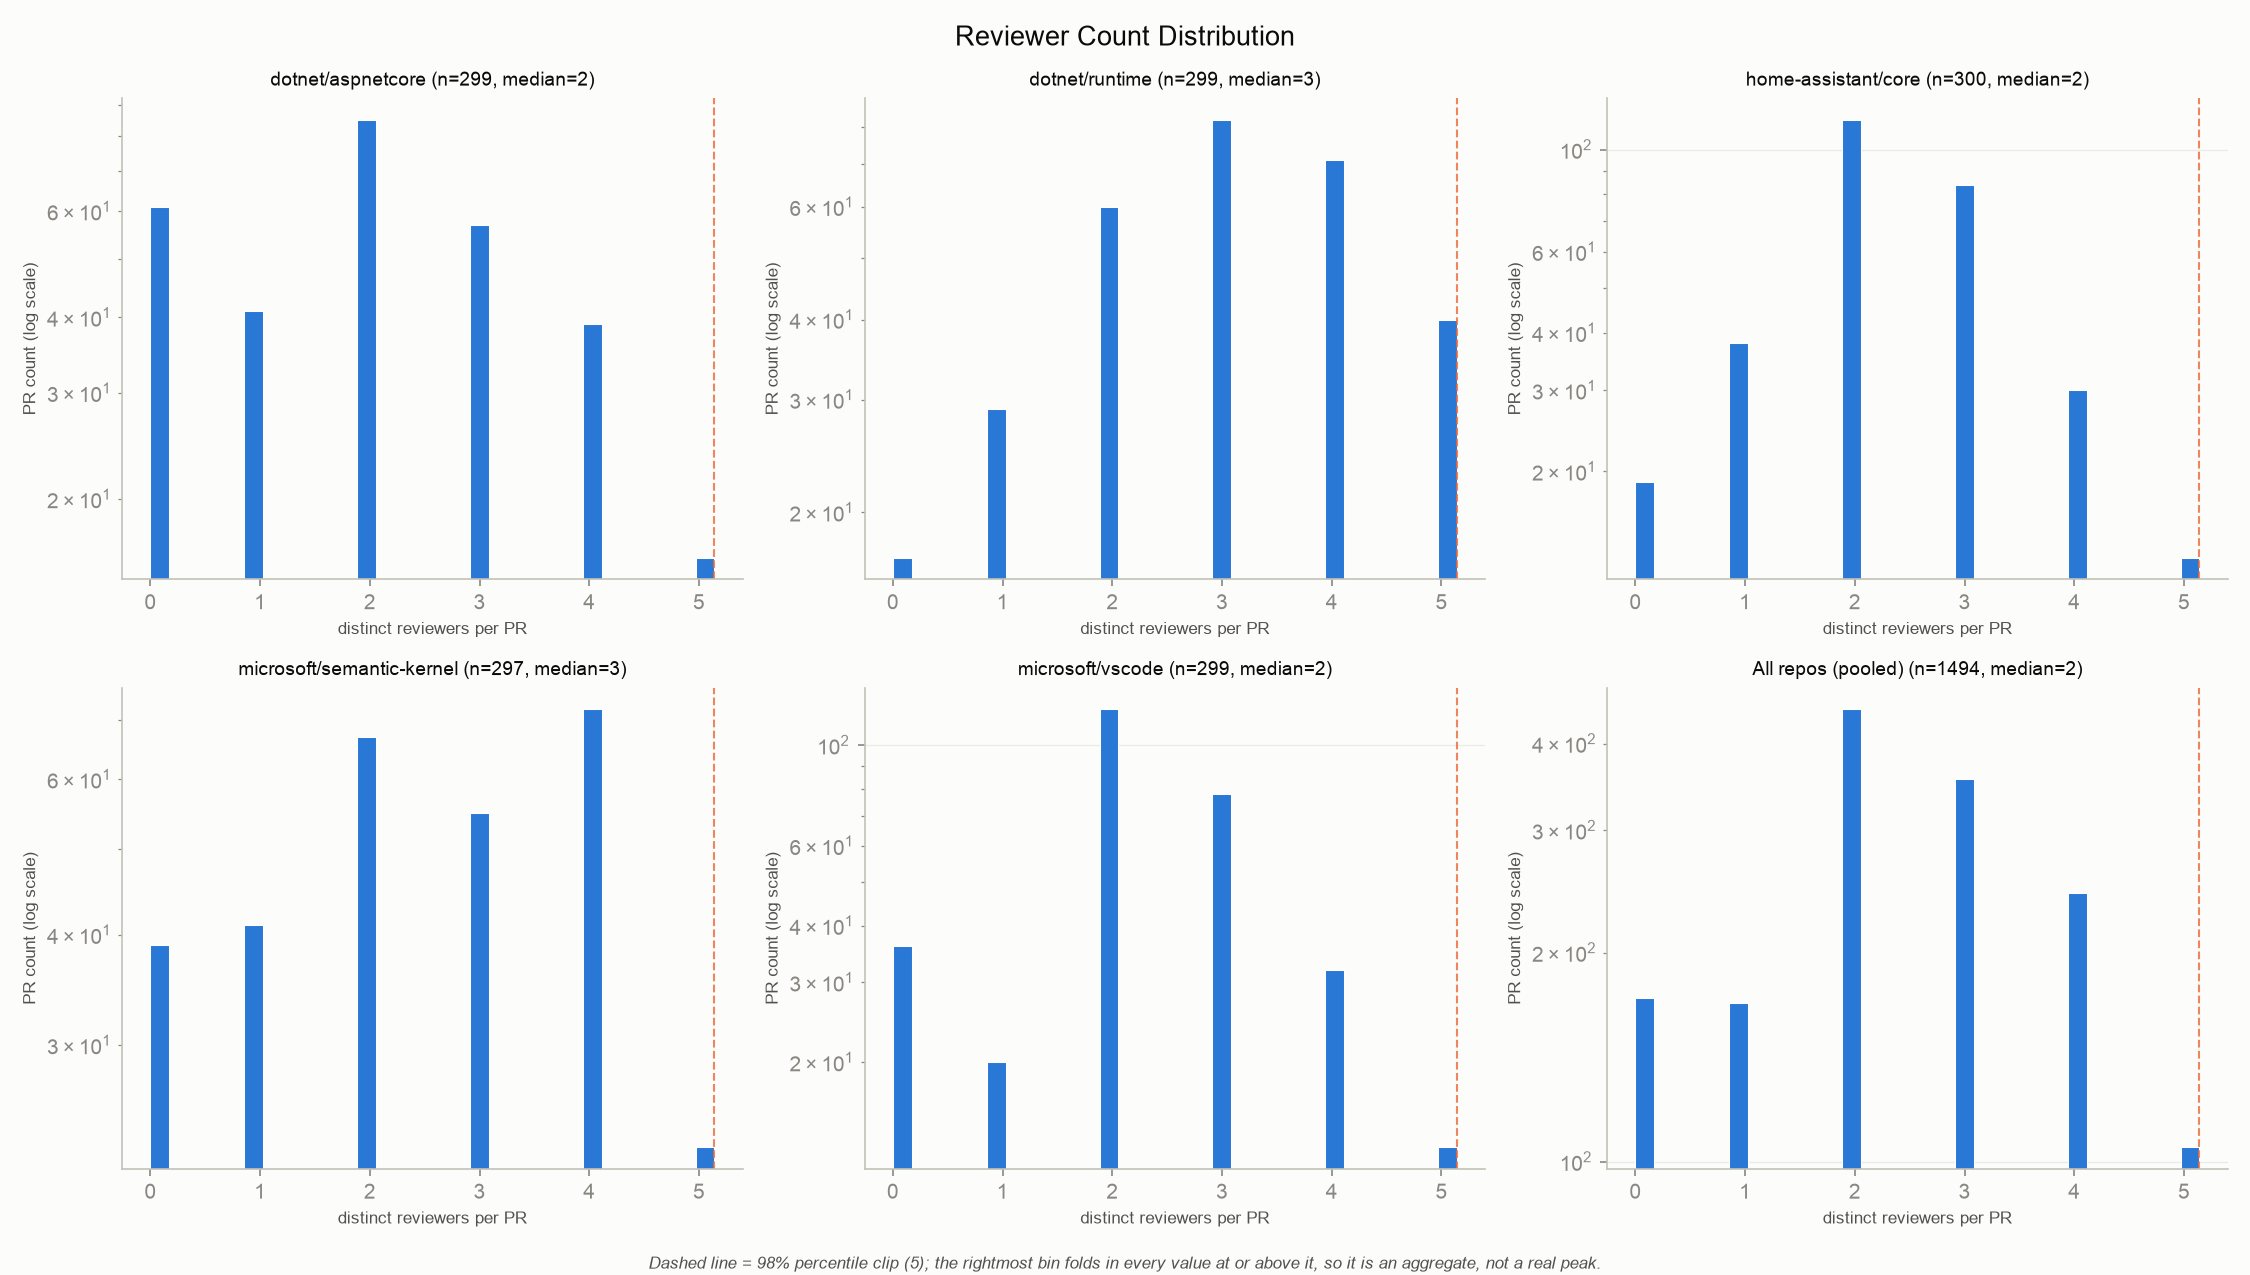
\includegraphics[width=0.92\textwidth]{../results/figures/reviewer_count_distribution.png}
\end{center}
\noindent\textbf{Figure 3.} Reviewer-count distribution per repo and pooled; most PRs cluster at
1--3 distinct reviewers.

\begin{center}
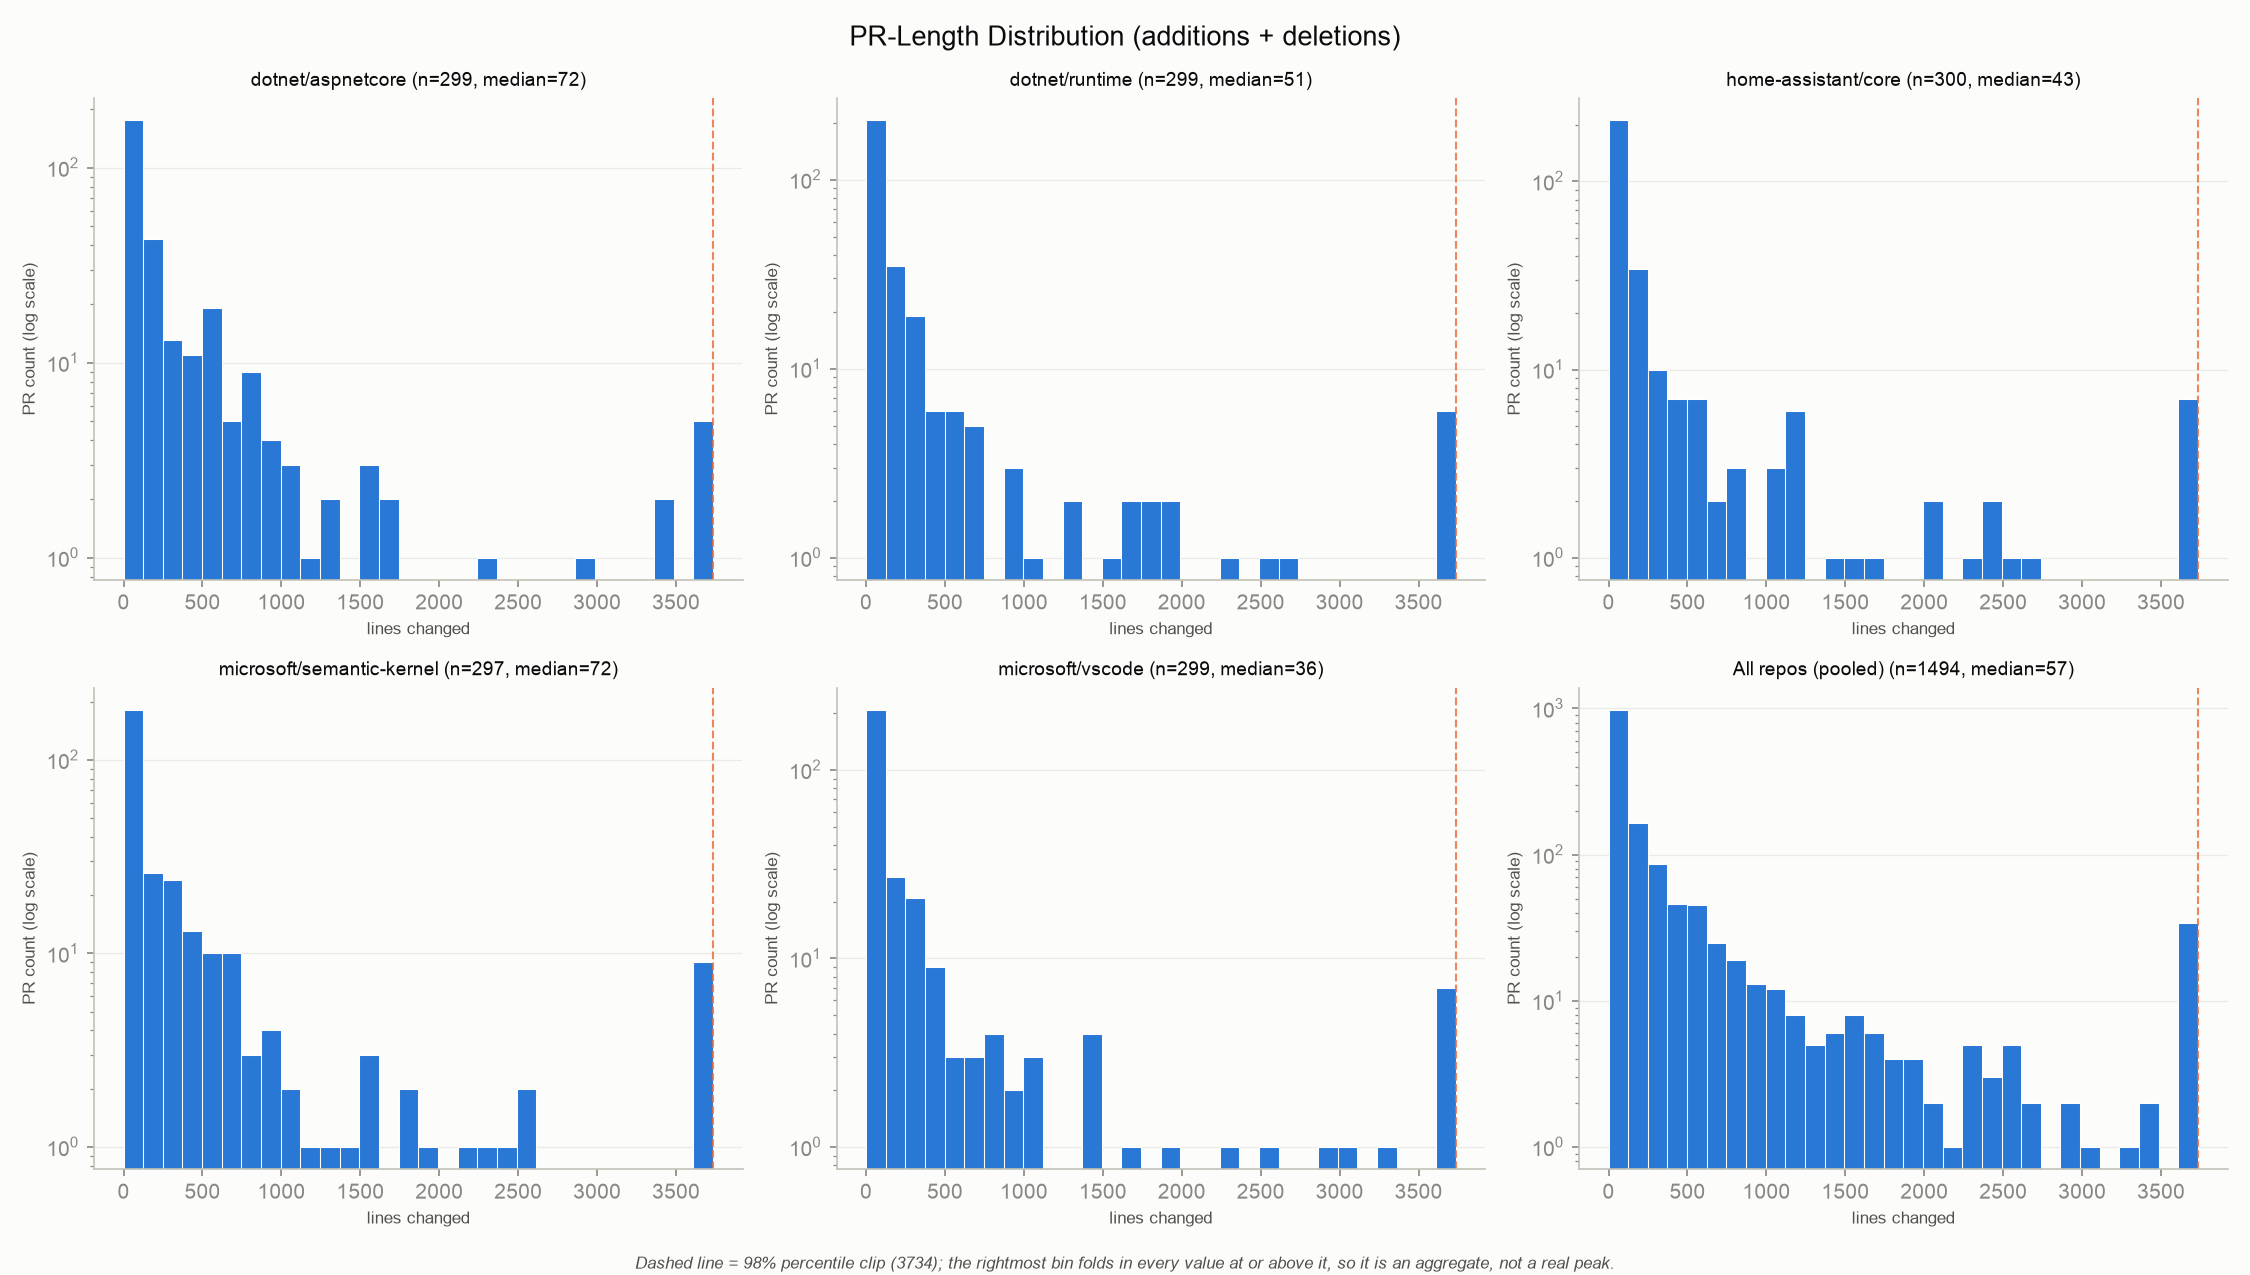
\includegraphics[width=0.92\textwidth]{../results/figures/pr_length_distribution.png}
\end{center}
\noindent\textbf{Figure 4.} PR-length (additions + deletions) distribution, clipped and annotated
identically to Figure 2. Medians in the tens of lines across every repo, confirming most PRs are
small regardless of repository.

\begin{center}
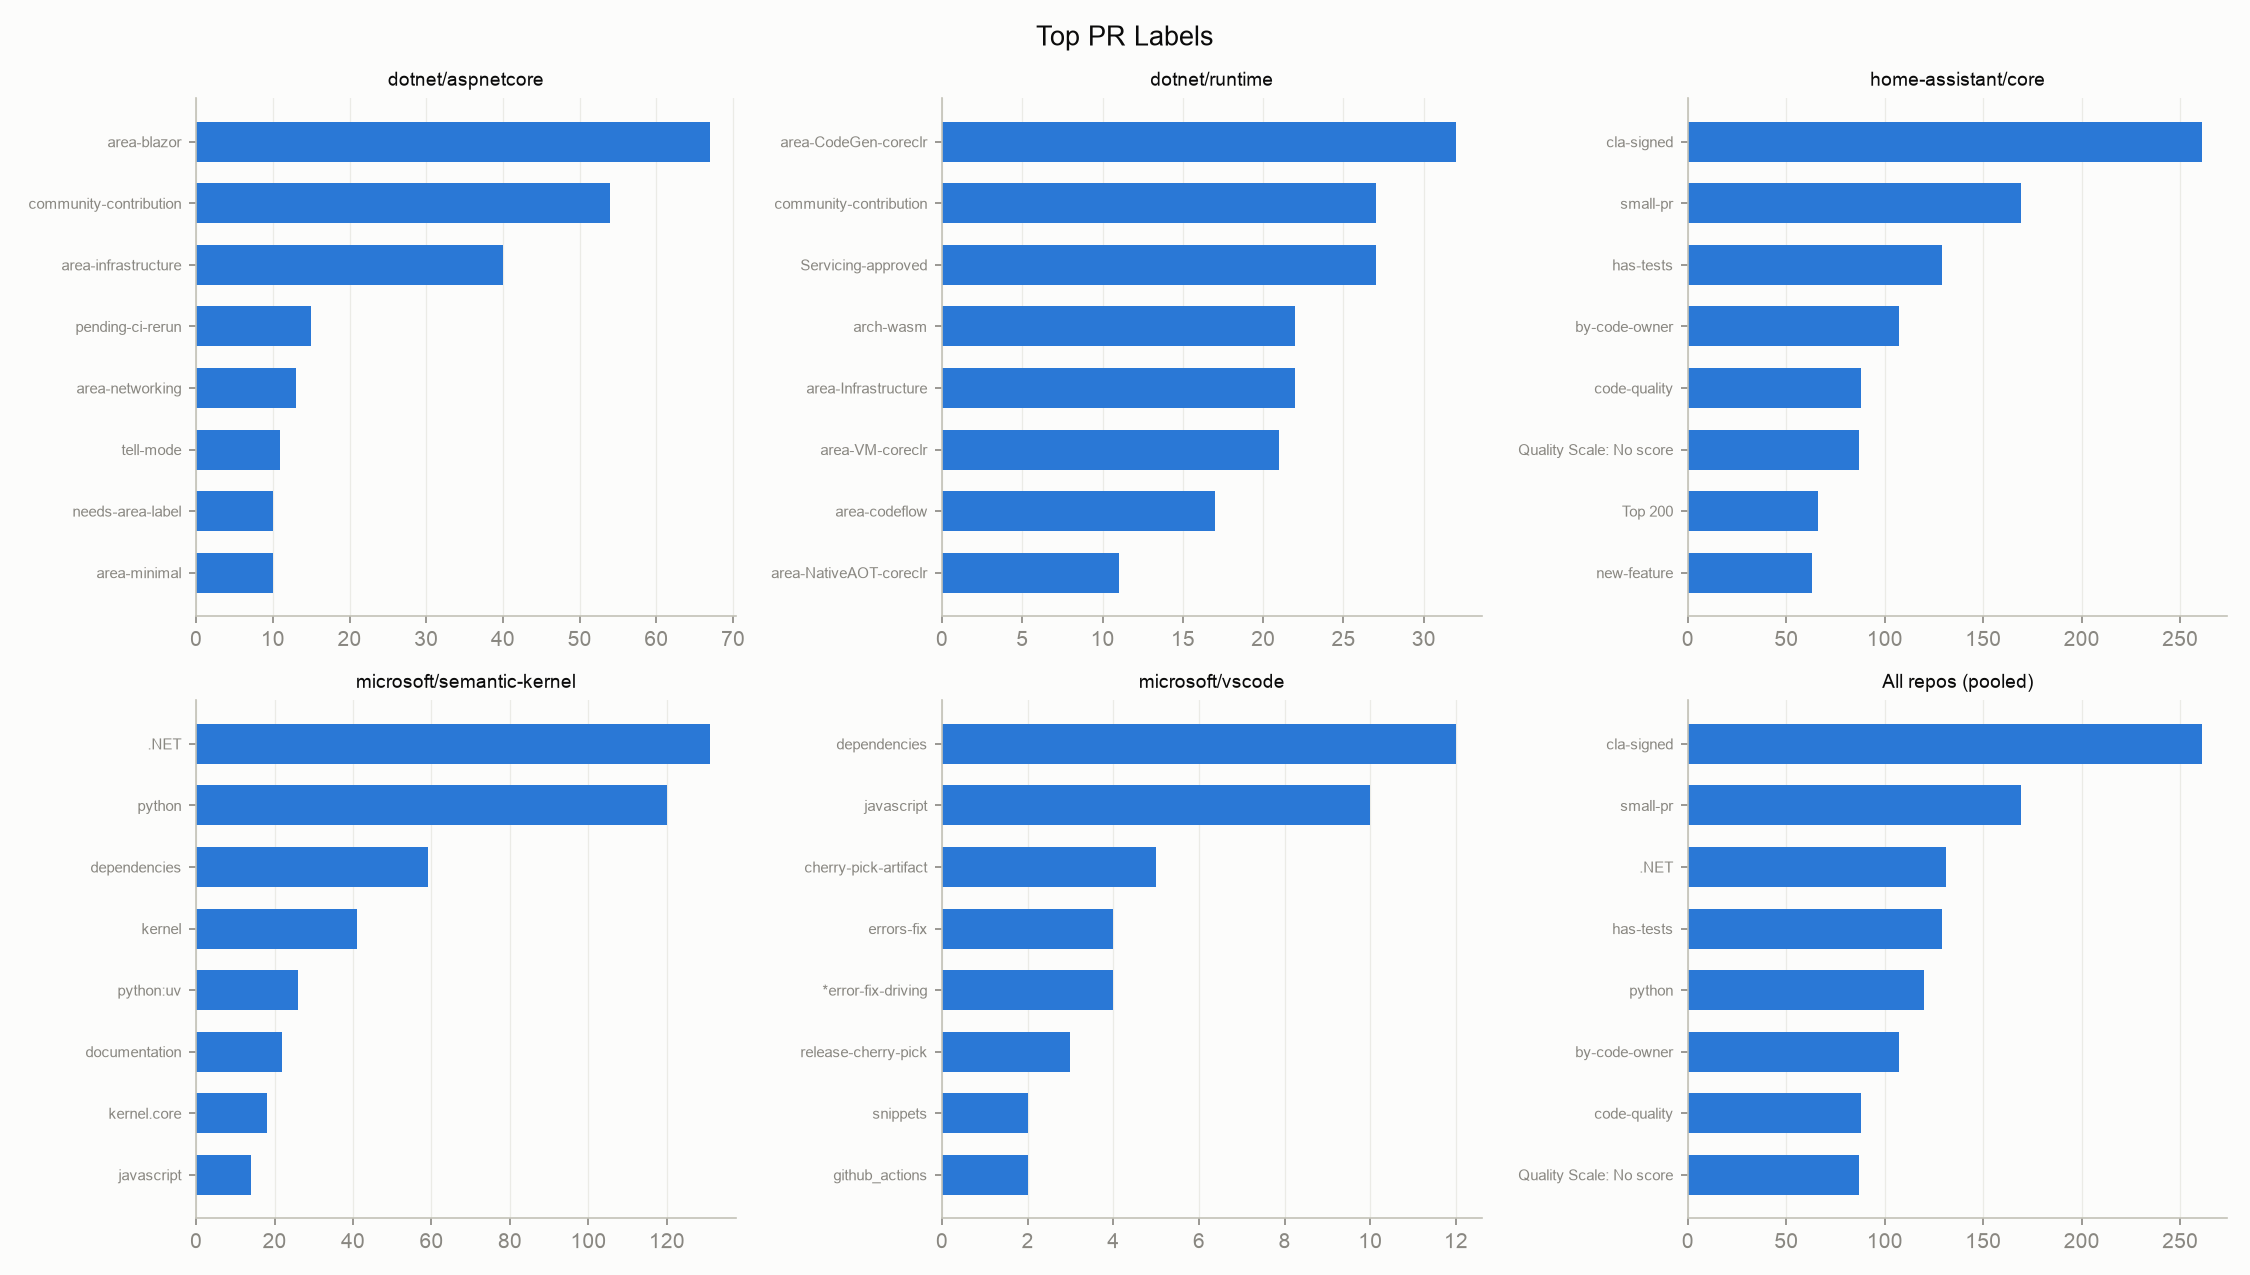
\includegraphics[width=0.92\textwidth]{../results/figures/label_distribution.png}
\end{center}
\noindent\textbf{Figure 5.} Top PR labels per repo and pooled. Visually confirms label usage is a
per-repository convention: \texttt{home-assistant/core}'s labels dominate the pooled panel purely
because that repo labels far more heavily, not because those labels are meaningful project-wide.

\begin{center}
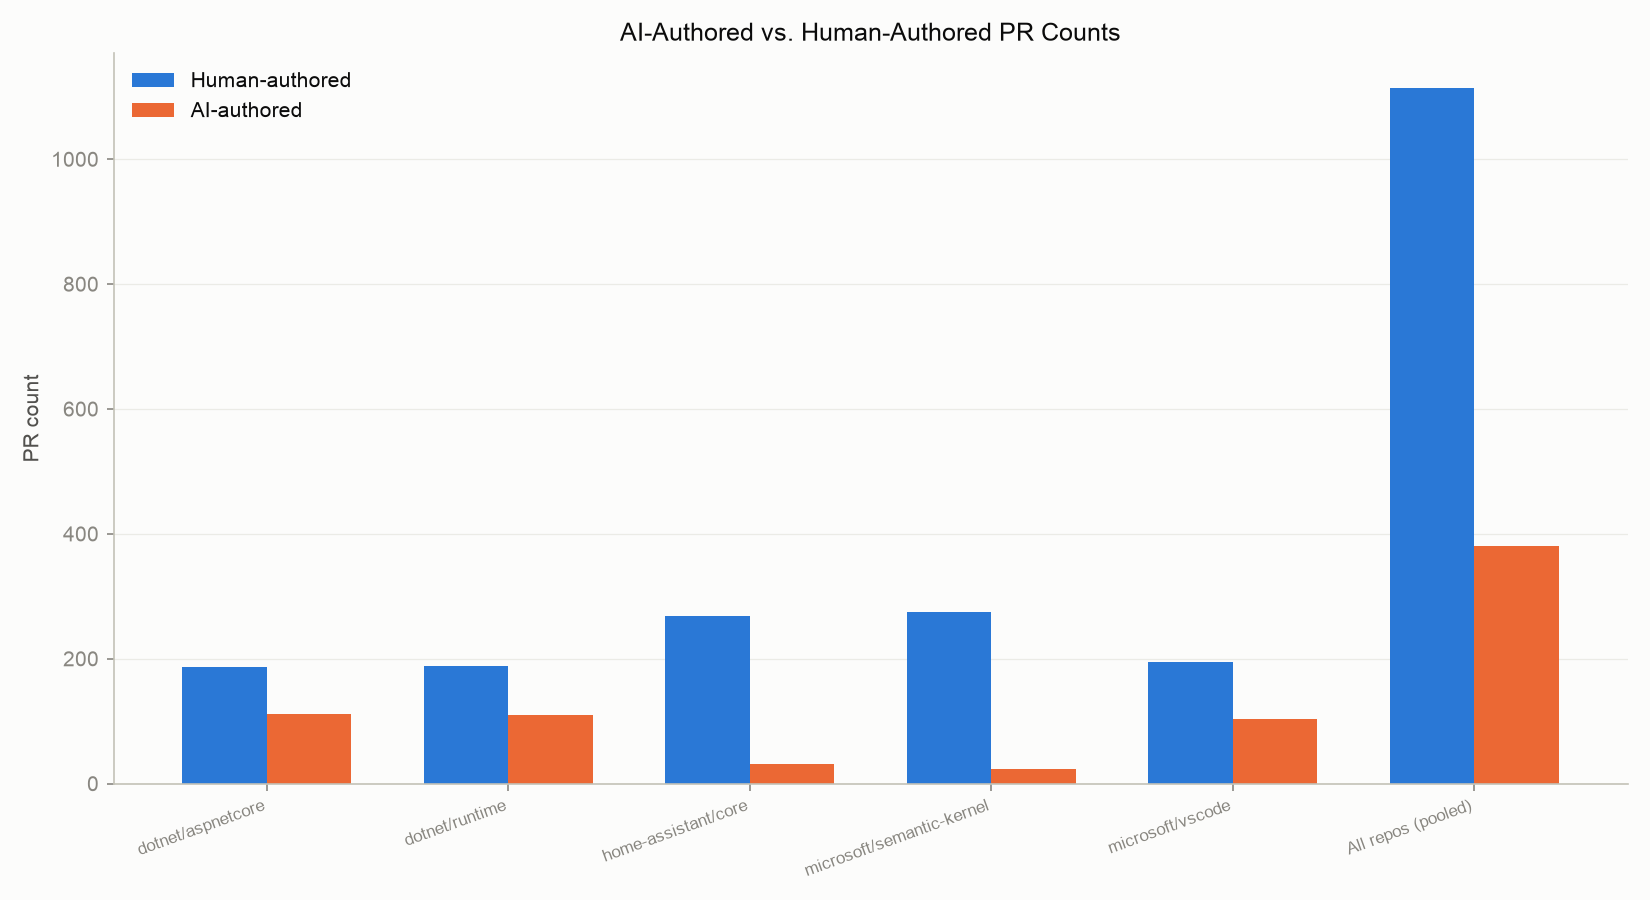
\includegraphics[width=0.92\textwidth]{../results/figures/ai_vs_human_counts_per_repo.png}
\end{center}
\noindent\textbf{Figure 6.} AI-authored vs.\ human-authored PR counts per repo. Visually confirms
the large gap in AI-agent adoption between the two \texttt{dotnet} repos and
\texttt{microsoft/vscode} versus \texttt{home-assistant/core} and \texttt{semantic-kernel}.

\begin{center}
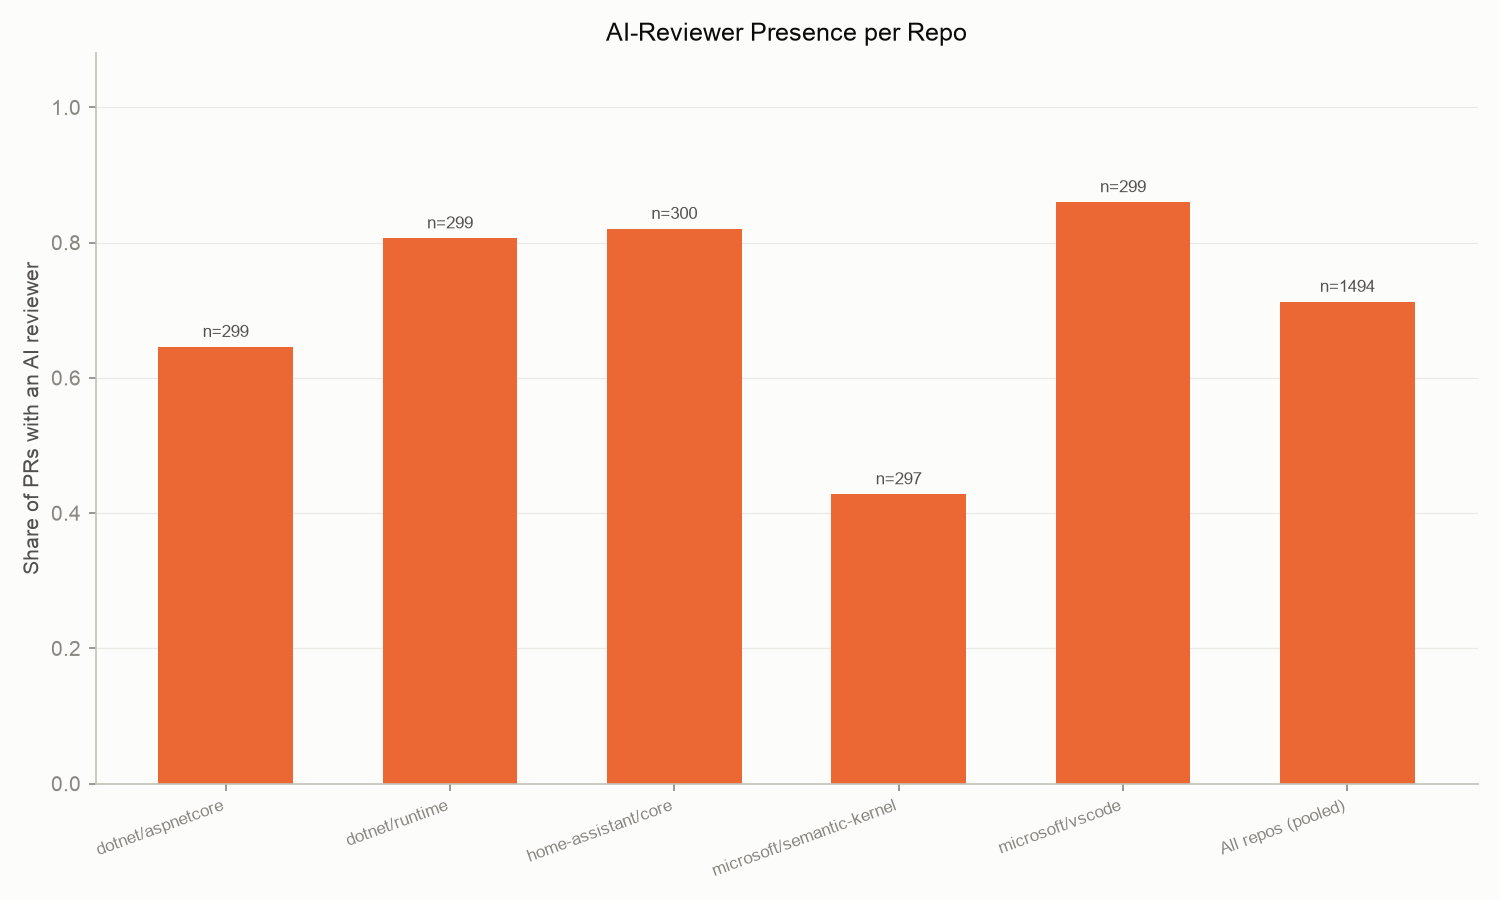
\includegraphics[width=0.92\textwidth]{../results/figures/ai_reviewer_presence_per_repo.png}
\end{center}
\noindent\textbf{Figure 7.} Share of PRs with an AI reviewer present, per repo, with sample size
annotated on every bar.

\begin{center}
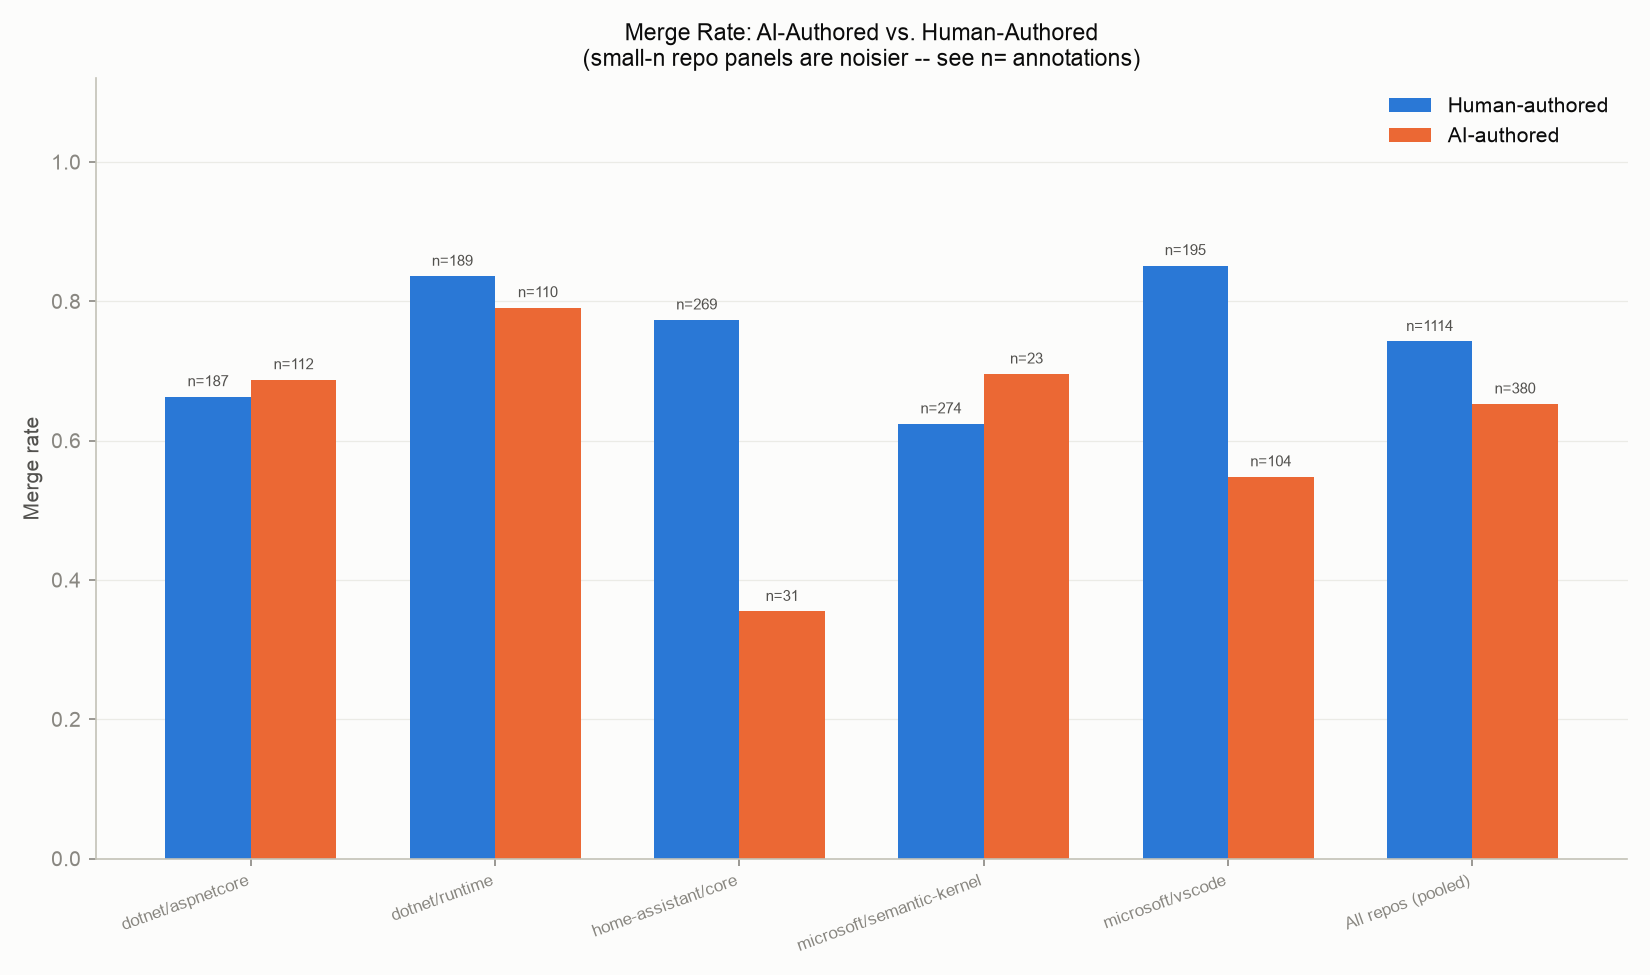
\includegraphics[width=0.92\textwidth]{../results/figures/merge_rate_ai_vs_human.png}
\end{center}
\noindent\textbf{Figure 8.} Merge rate, AI-authored vs.\ human-authored, per repo and pooled, with
$n$ annotated on every bar so the noisier small-sample repo panels (\texttt{semantic-kernel}
$n=23$, \texttt{home-assistant/core} $n=31$) are not read with the same confidence as the pooled
bar. This is the figure that makes the direction-flip described under ``Statistical Results''
visible at a glance.

}

%========================
% Summary of Issues
%========================

\experimentproblems{

\begin{enumerate}

\item \textbf{GitHub secondary rate limiting and transient server errors during mining.}
Fetching $\sim$1{,}500 PRs concurrently occasionally triggered HTTP 403 (secondary rate limit),
429, and 502 responses. \emph{Resolution:} exponential backoff with jitter, capped at 6 retry
attempts; GraphQL-level rate-limit errors (returned as HTTP 200 with an \texttt{errors} array)
were detected and retried separately from HTTP-level errors. 5 of 1{,}500 targeted PRs still
failed after exhausting retries (all confirmed genuine server-side 502s) and were excluded and
documented rather than retried indefinitely.

\item \textbf{Pagination-drift duplicate.} \texttt{microsoft/vscode\#326842} was fetched and
recorded twice. \emph{Root cause:} the ``recent closed PRs'' fill listing sorts by
\texttt{updated\_at} on a live, high-traffic repository; an item can shift position between two
sequential page fetches and land on both pages. \emph{Resolution:} defensive deduplication was
added at two layers --- the sampling logic (\texttt{build\_sample\_numbers}) and the fetch layer
(\texttt{GitHubClient.fetch\_prs}) --- and the already-mined dataset was rebuilt cleanly from the
existing on-disk cache (no new network calls needed, since every PR was already fetched at least
once).

\item \textbf{Schema gap masking genuinely distinct review comments as duplicates.} The
\texttt{review\_comments} and \texttt{issue\_comments} tables initially did not carry the
comment's own GraphQL node ID, so 12 rows with identical visible fields (same PR, same rounded
timestamp, similar body text) looked like accidental duplicates. \emph{Investigation:} the raw
cached JSON showed these were in fact three \emph{genuinely distinct} comment nodes --- GitHub's
Copilot reviewer had left three near-identical ``missing type annotation'' comments on three
different parameters in the same file. \emph{Resolution:} added a \texttt{comment\_id} column to
both tables, and added a \texttt{--rebuild-from-cache} mode to the mining script so all seven
tables could be regenerated from the disk cache without re-mining.

\item \textbf{Missing LaTeX toolchain / \texttt{ctexart.cls}.} The report template's class file
loads \texttt{ctexart}, a Chinese-typesetting class from the full \texttt{ctex} bundle, which is
unnecessary for a report written entirely in English and was not guaranteed to be present in a
minimal LaTeX install. \emph{Resolution:} a small local \texttt{ctexart.cls} shim
(\texttt{reports/ctexart.cls}) subclasses plain \texttt{article} and defines only the handful of
commands \texttt{experimentreport.cls} actually calls (\texttt{\textbackslash zihao\{n\}} as a
font-size mapping, \texttt{\textbackslash heiti} as \texttt{\textbackslash bfseries},
\texttt{\textbackslash chinese\{counter\}} as \texttt{\textbackslash arabic\{counter\}}), avoiding
the need to install real CJK support.

\end{enumerate}

}

%========================
% Reflections
%========================

\experimentexperience{

\textbf{(1) What are the differences between a Pull Request and a commit?}

A commit is an atomic, immutable snapshot of a set of file changes with a message and an author,
identified by a content hash (\texttt{sha}) --- it is a Git-level object with no notion of review
or merge status. A Pull Request is a GitHub-level, mutable social/workflow object that
\emph{groups one or more commits} together for review: it has its own title, description, labels,
reviewers, discussion threads, and a final merge/close decision, and it can be updated with new
commits after opening. In our data model this is exactly reflected in the table relationships:
each row in \texttt{pull\_requests} is a single mutable review unit, while \texttt{commits} is a
child table keyed by \texttt{pr\_id} with a many-to-one relationship --- our 1{,}494 mined PRs
carry 6{,}861 commits between them, an average of 4.59 commits per PR, and that ratio varies
by repository (PRs get amended with follow-up commits addressing review feedback, which a bare
commit has no equivalent of).

\textbf{(2) Why does code review improve software quality?}

Code review improves quality through several mechanisms visible in our own data: it catches
defects before they reach the main branch (a second pair of eyes reading unfamiliar code finds
issues the author, anchored to their own mental model, tends to miss); it enforces consistency
(e.g.\ the observed human reviewer comment ``the same issue at line 79 (for consistency)'' is
literally a consistency-enforcement act); and it transfers knowledge across the team (review
threads are a running record of design rationale). Our AI-reviewer example --- flagging a concrete
\texttt{StopIteration} crash risk from a missing dictionary key --- shows the same defect-catching
mechanism operating automatically at scale: 71.2\% of our mined PRs had at least one AI reviewer
touch them, meaning a large fraction of this dataset now gets an automated first-pass review layer
in addition to human review, not instead of it.

\textbf{(3) In what practical scenarios can merge prediction be applied?}

Concretely: (a) \emph{maintainer triage} --- surfacing PRs predicted unlikely to merge for early,
low-cost feedback to the contributor rather than a long silent wait; (b) \emph{CI/CD resource
allocation} --- prioritizing expensive test/build resources toward PRs likely to actually land;
(c) \emph{contributor-facing feedback tooling} --- warning a contributor before they even open a
PR that similar changes historically merge at a low rate in this repository; (d) \emph{backlog
health monitoring} --- our own per-repo merge rates already range from 63.0\% to 81.9\%, so a
maintainer team could use a predictive model to distinguish ``this PR looks like our typical
successful PR'' from ``this PR's characteristics resemble our historically-rejected PRs,'' which a
flat repository-wide prior cannot do.

\textbf{(4) What are the potential differences in review approaches between AI reviewers and
human reviewers?}

Our own retrieved examples show this concretely rather than abstractly. The AI reviewer comment
(``Guard against missing \texttt{DEFAULT\_CLOUD}\ldots to avoid \texttt{StopIteration} and a
crashed config flow'') is a single-shot, self-contained technical observation naming a specific
failure mode --- consistent with an LLM pattern-matching against the diff in isolation. The human
comments in our sample are conversational turns embedded in back-and-forth (``Thanks for the
feedback! I'll remove it.'') or reference project-wide context beyond the current diff (``along
with the same issue at line 79, for consistency'' --- a cross-reference a purely diff-scoped
reviewer would need explicit context to make). This matches the broader pattern the AI-detection
work surfaced: \texttt{copilot-pull-request-reviewer} is present on all 1{,}064 of our 1{,}064
AI-reviewed PRs, suggesting a fairly uniform, high-volume automated commenting style, whereas
human review style varies by reviewer and often carries social/negotiating content that a
diff-only signal would miss --- directly motivating Experiment 3/4's inclusion of PR description,
commit message, and repository-level context beyond the raw diff.

\textbf{(5) Does the dataset suffer from class imbalance? How can this be addressed?}

Yes: the pooled merge rate is 72.0\% merged vs.\ 28.0\% not merged (1{,}075 vs.\ 419), and the
imbalance is not even uniform --- it ranges from 63.0\% (\texttt{semantic-kernel}) to 81.9\%
(\texttt{dotnet/runtime}) by repository. This is a moderate but real imbalance: a trivial
always-predict-merged classifier would already score 72.0\% accuracy, making raw accuracy a
misleading metric on its own. This will be addressed in Experiment 2 by: (a) using a time-based
train/test split rather than a random split, to avoid look-ahead leakage in addition to the
class-balance question; (b) training with \texttt{class\_weight='balanced'} and comparing against
the unweighted model; (c) reporting precision/recall/F1 per class --- specifically minority-class
(not-merged) recall --- rather than accuracy alone, since accuracy alone would let a model that
never predicts ``not merged'' look artificially strong on this dataset.

}

%========================
% Instructor Comments
%========================

\teachercomment

\end{document}
